\section{視覚と行動の end-to-end 学習により経路追従行動をオンラ
インで模倣する手法}
岡田らの手法では,メトリックマップに基づく経路追従行動を視覚を入力とした行動へ模倣するために,end-to-end学習を用いた手法を提案している.
ロボットは経路を自律移動するのと同時に学習を行う.

訓練時には,ROS の navigation パッケージを使用して,設定した経路を追従する.
その際,ロボットに取り付けたカメラから取得したRGB画像とルールベース制御器が出力するヨー方向の角速度をペアにして,0.2秒の周期でデータセットに追加する.
訓練時,訓練後ともに並進速度は0.2m/sに固定し,カメラ画像は64×48にリサイズする.
次に,このデータセットからバッチサイズ8で教師データを抽出し,end-to-end学習を行う.
このデータ収集から学習までの一連の流れを1ステップと定義している.
収集には3台のカメラを使用することで,データの多様性を高めるとともに過学習を防ぐ効果を狙っている.
左右のカメラ画像に対するヨー方向の角速度には経路復帰を補助するためのオフセット(±0.2rad/s)を加える.

\clearpage
\begin{figure}[htbp]
  \centering
   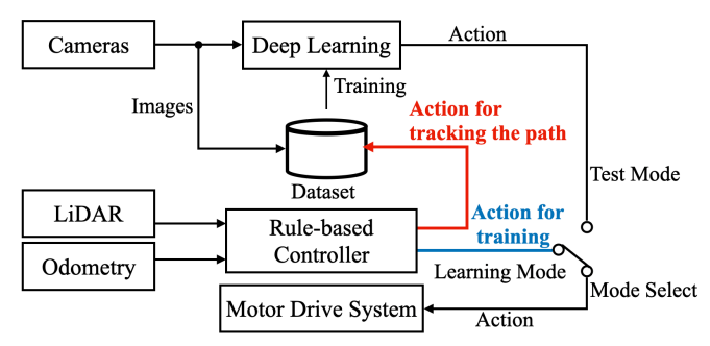
\includegraphics[width=110mm]{images/pdf/okada/method_sys.pdf}
   \caption[Structure of the Okada and others proposed system]{Structure of the Okada and others proposed system(Quoted from\cite{okada2020})}
   \label{fig:okada_sys}
\end{figure}

学習器の訓練後は,中央のカメラから得たRGB画像を入力とし,出力されるヨー方向の角速度を用いて経路を追従する.
この手法により,学習した経路を,画像のみを入力とした学習器の出力で自律移動できることが確認されている.